% ---------------------------------------------------------------------------- %
\subsubsection*{Ziel}
% ---------------------------------------------------------------------------- %
Das Ziel ist  die Bestimmung der Parameter $K_{rk}$, $T_{nk}$  und $T_{vk}$ in
der \"Ubertragungsfunktion des Reglers:

\begin{equation} \label{eq:pid:target}
    H_{rpid} = K_{rk} \cdot \biggl[ \frac{(1 + s \cdot T_{nk}) \cdot (1 + s \cdot T_{vk}) }{ s \cdot T_{nk} } \biggr]
\end{equation}


% ---------------------------------------------------------------------------- %
\subsubsection{Bestimmung der Reglerfrequenz $\mathbf{\boldsymbol{\omega}_{pid}}$}
% ---------------------------------------------------------------------------- %

Analog  zum PI-Regler  wird  zuerst  im Phasengang  der  Strecke die  Frequenz
$\omega_{pid}$  bestimmt,  f\"ur  welche   die  Phase  einen  bestimmten  Wert
aufweist,  aber   im  Unterschied   zum  PI-Regler  wird   hier  $-135\degree$
benutzt\footnotemark[7]:

\begin{equation} \label{eq:pid:phi_s}
    \varphi_s(\omega_{pid}) = -135 \degree
\end{equation}

\footnotetext[7]{%
    Wie   auch  beim   PI-Regler   stellt  diese   Frequenz  lediglich   einen
    Ausgangspunkt dar  und kann  zur weiteren  Optimierung des  Resultats noch
    angepasst werden.
}

In unserem Beispiel ergibt dies:

\begin{equation} \label{eq:pid:omega_pid}
    \omega_{pid} = \SI{0.6714}{\per\second}
\end{equation}

Eine       graphische       \"Uberpr\"ufung        kann       anhand       von
Abbildung~\ref{fig:pid:complete} durchgef\"uhrt werden.


% ---------------------------------------------------------------------------- %
\subsubsection{Steigung des Phasengangs bei der Reglerfrequenz}
% ---------------------------------------------------------------------------- %

Anschliessend   wird   die   Steigung    des   Phasengangs   $\varphi_s$   der
Strecke  bei  der   Frequenz  $\omega_{pid}$  bestimmt. Ausgangspunkt  daf\"ur
ist   die    \"Ubertragungsfunktion   der   Regelstrecke    (siehe   Gleichung
\ref{eq:transfer:plant}).

\begin{equation} \label{eq:transfer:plant:derivative}
    \frac{d\varphi_s}{d\omega} \biggr \rvert_{\omega=\omega_{pid}}
        = \frac{d(arg(H_s(j\omega)))}{d\omega} \biggr \rvert_{\omega=\omega_{pid}}
        = \SI{-1.5124}{\second}
\end{equation}
\todo{Einheit \"uberpr\"ufen}


% ---------------------------------------------------------------------------- %
\subsubsection{Hilfsparameter $\boldsymbol{\beta}$}
% ---------------------------------------------------------------------------- %

Zwischen  den Steigungen  der Phasen  des offenen  Regelkreises ($\varphi_o$),
der  Strecke  ($\varphi_s$)  und   des  Reglers  ($\varphi_r$)  gilt  gem\"ass
Tabelle~\ref{tab:terms} folgende Beziehung:

\begin{equation} \label{eq:pid:phi_sum}
    \varphi_o = \varphi_s + \varphi_r
\end{equation}

Da die Ableitung eine lineare Funktion ist, gilt somit auch:
\begin{equation} \label{eq:pid:dphi_sum}
    \frac{d\varphi_o}{d\omega} = \frac{d\varphi_s}{d\omega} + \frac{d\varphi_r}{d\omega}
\end{equation}

Diese Beziehungen  k\"onnen auch  gut in Abbildung  \ref{fig:pid:complete} von
Hand \"uberpr\"uft werden.

Es soll nun gelten:

\begin{equation} \label{eq:pid:dphi_o_target}
    \frac{d\varphi_o}{d\omega} \biggr \rvert_{\omega=\omega_{pid}} = - \frac{1}{2}
\end{equation}

Da   $\frac{d\varphi_s}{d\omega}$  durch   die  Strecke   gegeben  und   somit
unver\"anderlich ist, kann lediglich der Wert von $\frac{d\varphi_r}{d\omega}$
angepasst werden, damit Gleichung~\ref{eq:pid:dphi_o_target} erf\"ullt wird.

Dazu f\"uhrt man den Hilfsparameter $\beta$ ein, f\"ur den gilt:

\begin{gather} \label{eq:pid:beta:start}
    \begin{split}
        \frac{1}{T_{vk}} & = \frac{\omega_{pid}}{\beta} \\
        \frac{1}{T_{nk}} & = \omega_{pid} \cdot \beta  \\
                       0 & <  \beta \leq 1
    \end{split}
\end{gather}

Wie in Abbildung  ~\ref{fig:pid:complete} gesehen werden kann\footnotemark[8],
liegen  die   beiden  Frequenzen  $\frac{1}{T_{vk}}$   und  $\frac{1}{T_{nk}}$
symmetrisch um  den Faktor $\beta$ respektive  $\frac{1}{\beta}$ oberhalb bzw.
unterhalb der Frequenz $\omega_{pid}$.

\footnotetext[8]{%
    Man  beachte  dabei,  dass  der Plot  logarithmisch  skaliert  ist.   Eine
    identische Wegstrecke  zwischen zwei  Punkte-Paaren auf  der Frequenzachse
    bedeutet also,  dass diese um denselben  \emph{Faktor} auseinander liegen,
    und nicht,  dass die Differenz  zwischen den jeweiligen  Punkten identisch
    ist. Im  Falle  der  Punkte-Paare $[\frac{1}{T_{nk}},  \omega_{pid}]$  und
    $[\omega_{pid}, \frac{1}{T_{vk}}]$  ist  dieser  Faktor  $\beta$,  wie  in
    Gleichung~\ref{eq:pid:beta:start} ersichtlich.
}


Will man $\beta$ von Hand  berechnen, trifft man zuerst eine ``vern\"unftige''
Annahme, zum Beispiel:

\begin{equation} \label{eq:pid:beta:initial_value}
    \beta = 0.5
\end{equation}

Mit  diesem Startwert  bestimmt  man nun  $T_{nk}$  und ${T_{vk}}$:

\begin{gather} \label{eq:pid:t_nk_t_vk_initial_results}
    \begin{split}
        {T_{vk}} & = \frac{\beta}{\omega_{pid}}  = \frac{0.5}{\SI{0.6714}{\per\second}}                   = \SI{0.7447}{\second} \\
        {T_{nk}} & = \frac{1}{\omega_{pid} \cdot \beta} = \frac{1}{\SI{0.6714}{\per\second} \cdot 0.5 }  = \SI{2.9789}{\second} \\
    \end{split}
\end{gather}

Die  somit  erhaltenen  Werte   setzt  man  in  Gleichung  \ref{eq:pid:target}
ein,   zusammen   mit   dem    Wert   f\"ur   $\omega_{pid}$   aus   Gleichung
\ref{eq:pid:omega_pid}. Da  $K_{rk}$   noch  unbekannt   ist,  aber   auf  den
Phasengang  keinen  Einfluss   hat,  setzt  man  vorerst  $K_{rk}   =  1$,  um
weiterrechnen zu k\"onnen.

\begin{gather} \label{eq:pid:t_nk_t_vk_initial_results}
    \begin{split}
        H_{rpid} & = K_{rk} \cdot \biggl[ \frac{(1 + j\omega \cdot T_{nk}) \cdot (1 + j\omega \cdot T_{vk}) }{ j\omega \cdot T_{nk} } \biggr] \\
                 & = 1      \cdot \biggl[ \frac{(1 + j\omega \cdot \SI{2.9789}{\second}) \cdot (1 + j\omega \cdot \SI{0.7447}{\second}) }{ j\omega \cdot  \SI{2.9789}{\second}} \biggr]
    \end{split}
\end{gather}

Von dieser Gleichung bestimmt man nun  den Phasengang und wertet danach dessen
Ableitung an der Stelle $\omega = \omega_{pid}$ aus. Die zugeh\"orige Rechnung
kann in Anhang~\ref{app:beta} gefunden werden.

\begin{gather} \label{eq:pid:phi_r_first_iteration}
    \begin{split}
        \varphi_r (j\omega)                                            & = arg(H_{rpid}(j\omega))        \\
        \frac{d\varphi_r}{d\omega} \biggr \rvert_{\omega=\omega_{pid}} & = \SI{1.1920}{\second}
    \end{split}
\end{gather}


Setzt man dies in Gleichung \ref{eq:pid:phi_sum} ein, erh\"alt man:
\begin{gather} \label{eq:pid:phi_sum_result_iteration_one}
    \begin{split}
    \frac{d\varphi_o}{d\omega}       \biggr \rvert_{\omega=\omega_{pid}, \beta=0.5}
        & = \frac{d\varphi_s}{d\omega} \biggr \rvert_{\omega=\omega_{pid}}
        + \frac{d\varphi_r}{d\omega} \biggr \rvert_{\omega=\omega_{pid}, \beta=0.5} \\
        & = \SI{-1.5124}{\second} + \SI{1.1920}{\second} \\
        & = \SI{-0.3204}{\second} \\
        & > -\frac{1}{2}
    \end{split}
\end{gather}

Mit  $\beta  = 0.5$  erh\"alt  man  also eine  zu  hohe  Steigung des  offenen
Regelkreises   an    der   Stelle  $\omega_{pid}$,   folglich   muss   $\beta$
\emph{verkleinert} werden.   Diese Berechnungen  werden nun mit  jeweils neuen
Werten  f\"ur  $\beta$  solange  wiederholt,  bis  die  Steigung  des  offenen
Regelkreises die gew\"unschte N\"ahe zu $-\frac{1}{2}$ aufweist.

Da die manuelle Iteration dieses Prozesses  enorm viel Zeit in Anspruch nimmt,
bietet  sich  hier  eine  Automatisierung  an. Die  Berechnung  mittels  eines
geeigneten Algorithmus in Matlab liefert schlussendlich folgendes Ergebnis:

\begin{gather} \label{eq:pid:beta_result}
    \begin{split}
        \beta    & = 0.2776 \\
        {T_{vk}} & = \frac{\beta}{\omega_{pid}}           = \SI{0.4134}{\second} \\
        {T_{nk}} & = \frac{1}{\omega_{pid} \cdot \beta}   = \SI{5.3656}{\second} \\
    \end{split}
\end{gather}

Diese Werte sind ebenfalls in Abbildung~\ref{fig:pid:complete} eingetragen.

Sollte  man  f\"ur  $\beta$  einen komplexen  Wert  erhalten,  wird  $\beta=1$
gesetzt.

Die zur  Bestimmung von $\beta$,  $T_{vk}$ und $T_{nk}$  benutzten Algorithmen
sind    in     Anhang~\ref{app:algo:slope}    respektive~\ref{app:algo:tnktvk}
dokumentiert.


% ---------------------------------------------------------------------------- %
\subsubsection{Durchtrittsfrequenz $\mathbf{\boldsymbol{\omega}_d}$}
% ---------------------------------------------------------------------------- %

Als  letzte Unbekannte  verbleibt  die Verst\"arkung  $K_{rk}$. Wie auch  beim
PI-Regler ist zum Finden  der Verst\"arkung die Durchtrittsfrequenz $\omega_d$
zu bestimmen, um anschliessend mit deren Hilfe $K_{rk}$ auszurechnen.

Die    Resultate    aus     Gleichung~\ref{eq:pid:beta_result}    werden    in
Gleichung~\ref{eq:pid:target} eingesetzt. $K_{rk}$  ist immer  noch unbekannt,
und wird daher vorerst bei 1 belassen.

\begin{gather} \label{eq:pid:h_rpid_beta_result}
    \begin{split}
        H_{rpid} & = K_{rk} \cdot \biggl[ \frac{(1 + s \cdot T_{nk}               ) \cdot (1 + s \cdot T_{vk}               ) }{ s \cdot T_{nk}               } \biggr]
                   = 1      \cdot \biggl[ \frac{(1 + s \cdot \SI{5.3656}{\second} ) \cdot (1 + s \cdot \SI{0.4134}{\second} ) }{ s \cdot \SI{5.3656}{\second} } \biggr]
    \end{split}
\end{gather}


Es interessiert hier der Phasengang des offenen Regelkreises (auch eingetragen
in   Abbildung~\ref{fig:pid:complete}),    wozu   die   \"Ubertragungsfunktion
der  Strecke   (siehe  Gleichung   \ref{eq:transfer:plant})  mit   der  soeben
bestimmten  provisorischen   \"Ubertragungsfunktion  des   Reglers  (Gleichung
\ref{eq:pid:h_rpid_beta_result}) multipliziert wird.

\begin{equation} \label{eq:pid:h_o_k_rk_one}
    H_{o}(j\omega) = H_{rpid}(j\omega) \cdot H_s(j\omega)
\end{equation}

Nun wird die  Durchtrittsfrequenz $\omega_d$ berechnet, an  welcher der offene
Regelkreis eine  Verst\"arkung von $\SI{0}{\decibel} =  1$ aufweisen soll. Wie
auch  beim  PI-Regler  werden  wir   hier  ein  \"Uberschwingen  von  $16.3\%$
anstreben, womit gem\"ass Tabelle \ref{tab:phi_s} gilt:

\begin{equation} \label{eq:pid:omega_d_target}
    \varphi_s(\omega_d) = \varphi_s = -128.5\degree
\end{equation}

Dieser   Wert   wird   analog   zum   PI-Regler   aus   dem   Phasengang   des
offenen Regelkreises  abgelesen (siehe Abbildung~\ref{fig:pid:complete}). Eine
Nachrechnung mittels Matlab ergibt:

\begin{equation} \label{eq:pid:omega_d_target}
    \omega_d = \SI{0.5341}{\per\second}
\end{equation}


% ---------------------------------------------------------------------------- %
\subsubsection{Bestimmung der Reglerverst\"arkung $\mathbf{K_{rk}}$}
% ---------------------------------------------------------------------------- %

Im letzten  Schritt wird  nun der Amplitudengang  des offenen  Regelkreises an
der  Stelle $\omega_d$  gleich 1  gesetzt  und diese  Gleichung nach  $K_{rk}$
aufgel\"ost:

\begin{equation} \label{eq:pid:h_o_k_rk_one}
    \begin{split}
        A_{o}(j\omega_d)    & = | H_{o}(j\omega_d) | = | H_{rpid}(j\omega_d) \cdot H_s(j\omega_d) |    \\
                            & = \Biggl \rvert
                                    K_{rk}
                                    \cdot
                                    \biggl[ \frac{(1 + j\omega_d \cdot T_{nk}) \cdot (1 + j\omega_d \cdot T_{vk}) }{ j\omega_d \cdot T_{nk} } \biggr] \Biggr \rvert \\
                            & \cdot
                                \Biggl \rvert
                                    K_s
                                    \cdot \frac{1}{1 + j\omega_d \cdot T_1}
                                    \cdot \frac{1}{1 + j\omega_d \cdot T_2}
                                    \cdot \frac{1}{1 + j\omega_d \cdot T_2}
                                    \Biggr \rvert \\
                            & = 1
    \end{split}
\end{equation}

Die einzusetzenden Werte sind:
\begin{gather} \label{eq:pid:h_o_k_rk_one}
    \begin{split}
        K_s         & = 2                        \\
        T_1         & = \SI{0.4134}{\second}     \\
        T_2         & = \SI{1.4894}{\second}     \\
        T_3         & = \SI{5.3655}{\second}     \\
        T_{nk}      & = \SI{5.3656}{\second}     \\
        T_{vk}      & = \SI{0.4134}{\second}     \\
        \omega_d    & = \SI{0.5341}{\per\second}
    \end{split}
\end{gather}

Womit man f\"ur die Verst\"arkung den Wert

\begin{equation} \label{eq:pid:k_rk_result}
    K_{rk} = 1.83084
\end{equation}

erh\"alt.


% ---------------------------------------------------------------------------- %
\subsubsection{Resultat}
% ---------------------------------------------------------------------------- %

Somit   ist  der   Regler   vollst\"andig  dimensioniert   und  hat   folgende
\"Ubertragungsfunktion:

\begin{equation} \label{eq:pid:result}
    H_{rpid}(s) = 1.83084 \cdot \biggl[ \frac{(1 + s \cdot \SI{5.3656}{\second} ) \cdot (1 + s \cdot \SI{0.4134}{\second} ) }{ s \cdot \SI{5.3656}{\second} } \biggr]
\end{equation}

Zusammenfassend sind in Abbildung~\ref{fig:pid:complete} die verschiedenen
Frequenzg\"ange und Frequenzen eingetragen.

\begin{figure}[h! width=\pagewidth]
    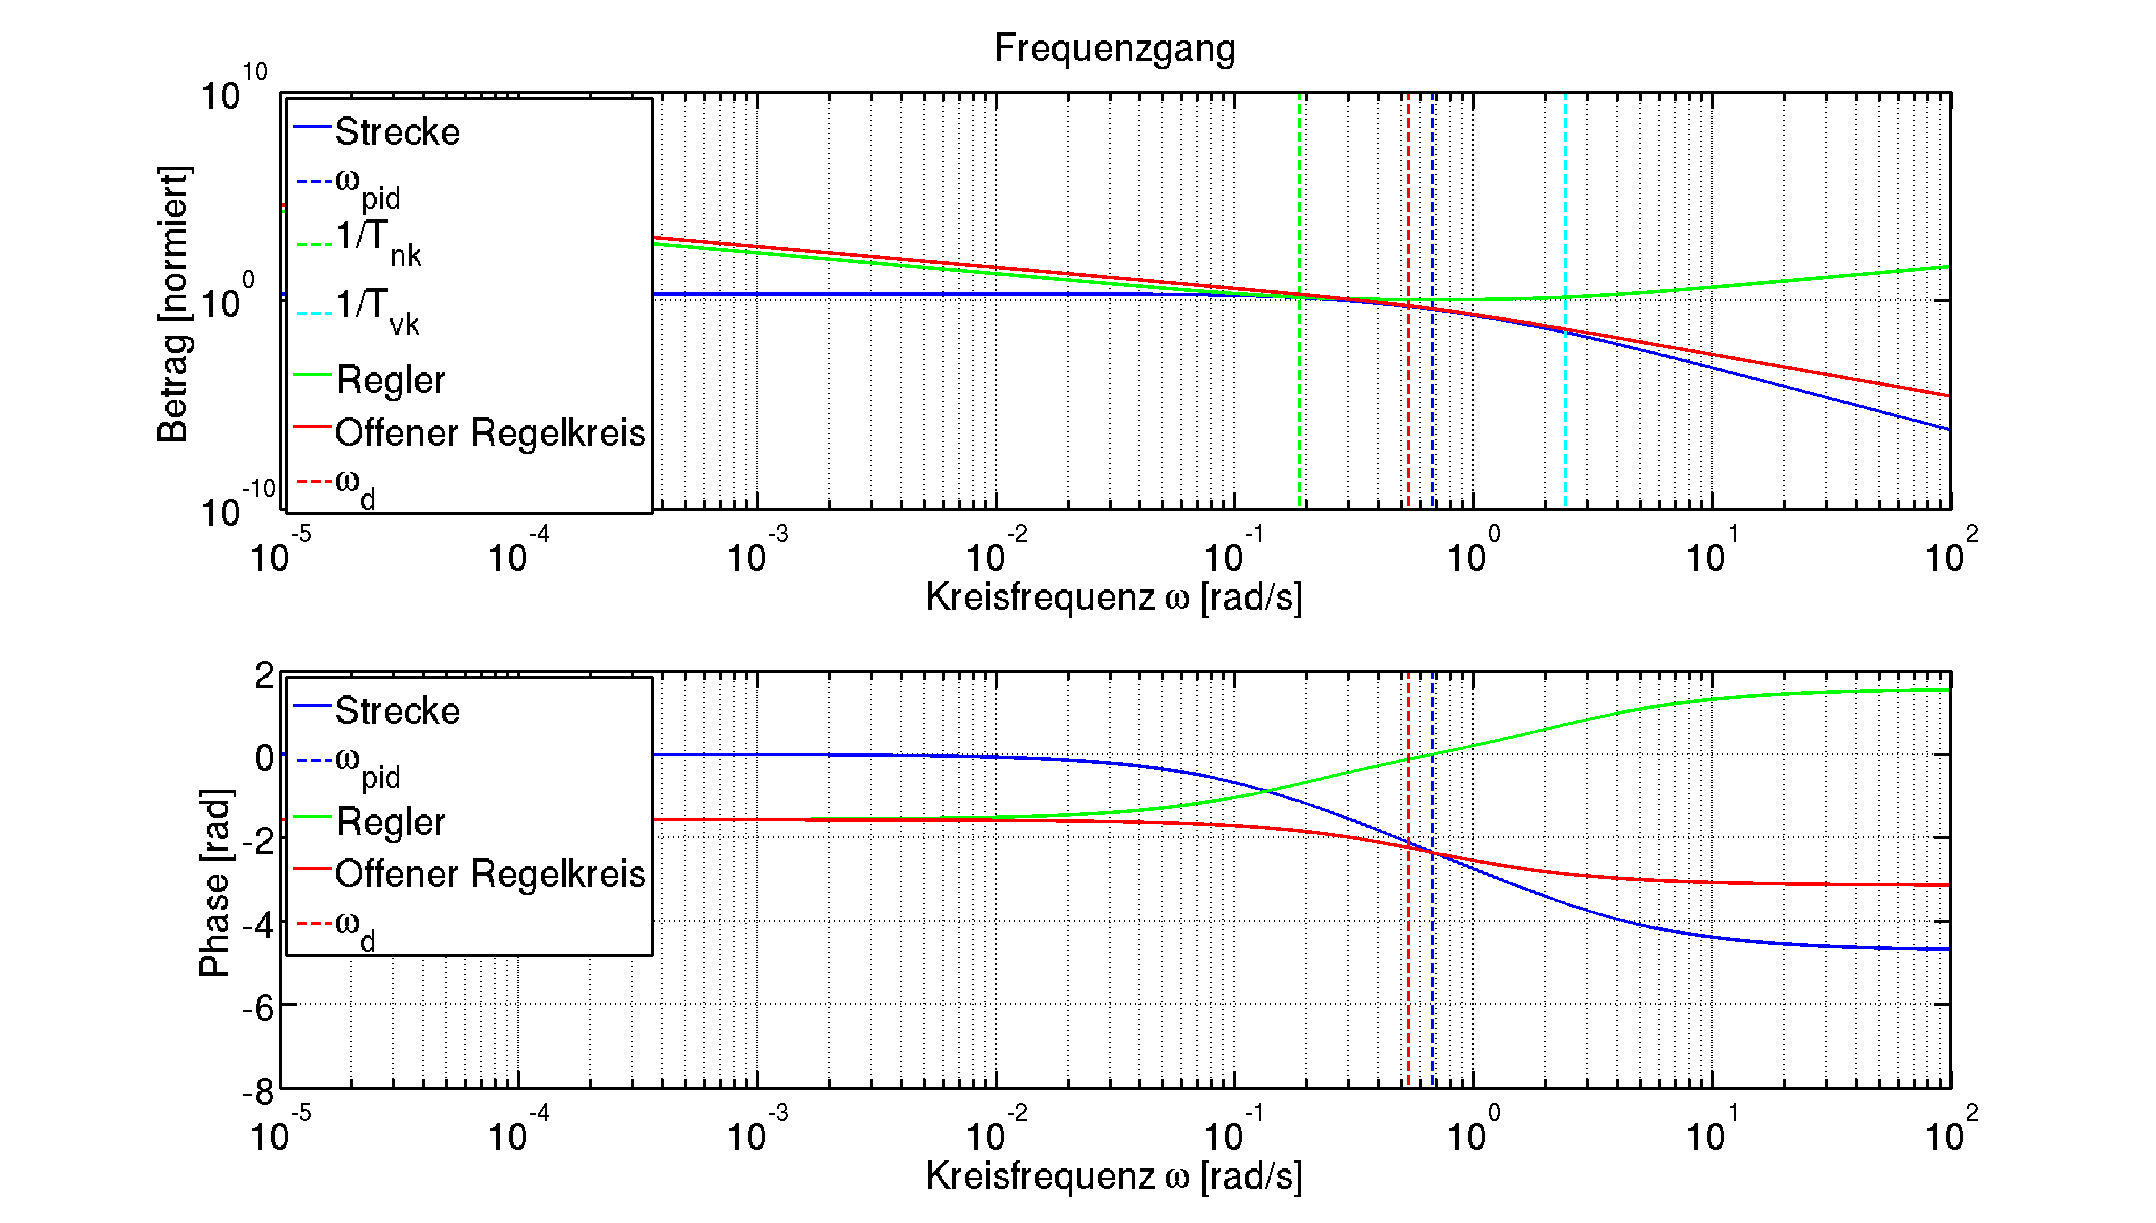
\includegraphics[width=\textwidth]{images/pidCompletePlot.png}
    \caption{%
        Frequenzgang der Strecke (blau), des  Reglers (gr\"un) und des offenen
        Regelkreises  (rot).  Ebenfalls  eingetragen  sind die  Reglerfrequenz
        $\omega_{pid}$,   die   beiden   Frequenzen   $\frac{1}{T_{vk}}$   und
        $\frac{1}{T_{nk}}$ sowie die Durchtrittsfrequenz $\omega_d$.
    }
    \label{fig:pid:complete}
\end{figure}
